%\documentclass{article}
%\usepackage{wasysym}
%\usepackage{graphicx}
%\usepackage{bm}
%\newcommand{\bc}{\begin{center}}
%\newcommand{\ec}{\end{center}}
%\newcommand{\be}{\begin{equation}}
%\newcommand{\ee}{\end{equation}}
%\newcommand{\bea}[1]{\begin{eqnarray}\label{#1}}
%\newcommand{\eea}{\end{eqnarray}}
%\newcommand{\bua}{\begin{eqnarray*}}
%\newcommand{\eua}{\end{eqnarray*}}
%\newcommand{\infint}{\int_{-\infty}^{\infty}}
%\newcommand{\dd}[2]{{{d#1}\over{d#2}}}
%\newcommand{\ddt}[1]{\dd{#1}{t}}
%\newcommand{\dddt}[1]{\dd{^2#1}{t^2}}
%\newcommand{\aver}[1]{\langle{#1}\rangle}
%\def\cl#1{{\cal #1}}               % for caligrafic letters
%\def\labs{\mid\!}
%\def\rabs{\!\mid}
%\begin{document}
%\setcounter{section}{5} No need for this when merging into main.
\section{Telescopes for visible light}

Astronomers use telescopes to collect radiation from astronomical sources and
to estimate their direction and structure as well as spectral and absolute 
intensities. The wide range of photon energies involved in astronomical 
observations means that the telescopes are very different in form depending
on wavelength band. We can subdivide telescope types roughly into four 
categories. 
\begin{itemize}
\item detectors which sense the direction of arrival and energy of individual
(gamma-ray) photons
\item non-focusing (X-ray) collimators which restrict the field of view of 
the detector
\item phased arrays, and pencil beam interferometers (metre wavelength)
\item reflecting or refracting telescopes which focus incoming radiation 
(all wavelengths except gamma-rays)
\end{itemize}
Here we will concentrate on the latter category, and especially to those 
telescopes used to observe visible and infra-red radiation. 
 
The theoretical
consideration of resolution that we discussed in previous lectures is only 
applicable if the lens or mirror as well as the intervening atmosphere
 is of sufficient optical quality that the image is not already degraded 
beyond the diffraction limit. There are many effects that will blur an image
and these are collectively known as aberrations. With one exception they 
can all effect images produced by both lenses or mirrors. The universal
or monochromatic aberrations are known as the Seidel aberrations. The 
exception is chromatic aberration and the related second order effects of 
transverse chromatic aberration and secondary color, and these only effect
lenses.

\subsection{Lenses, mirrors and geometric optics}

The speed of light in a vacuum is a constant, $c$, identical for all observers. 
The {\it phase velocity} $v$ of light in a dielectric medium such as air, water, or glass
is always less than $c$ such that
\[
n(\lambda)={c\over v(\lambda)}
\]
where $n$ is the {\it index of refraction}, which in general is a function of the 
wavelength $\lambda$. Another important characteristic of a material is thus the 
{\it chromatic dispersion} $dn/d\lambda$. Glassmakers traditionally express this
dispersion as the Abbe number, or costringence, defined in equation~\ref{eq:costringence}, 
which depends roughly on the reciprocal of the dispersion.

Along a ray of light moving through a medium (a homogenous medium will have straight rays
of light) one can measure the distance $s$ that light moves in time $t$
\[
s={ct\over n}
\]
Points of equal $s$ delineate a surface called the {\it geometrical wavefront}. Wavefronts
are always perpendicular to rays. If $ds$ is an infinitesimal element along a ray path the
ray travel time is 
\[
\tau=\int{ds\over v}={1\over c}\int nds={w\over c}
\]
where $w$ is the {\it optical path length}. In some situations with a coherent source (where
all waves are emitted in phase) the geometrical wavefronts also correspond to surfaces of
equal phase.

\subsubsection{Fermat's principle and Snell's law}

Fermat's principle states that the path of a ray between two points will always be an extremum
in total travel time $\tau$ or optical path length.

 Consider a situation where a plane separates
two different materials, and assume that the index of refraction is larger in the material on the
right. A light ray that travels towards the right will strike the normal to the surface at the 
{\it angle of incidence}, $\theta_1$, and the ray splits into two components - a reflected ray, 
and a refracted ray. These two rays make angles $\theta_R$ and $\theta_2$ with the normal, 
which is measured so that positive angles counterclockwise from the normal. 

Fermat's principle implies the law of reflection
\[
\theta_1=-\theta_R.
\]
We can also deduce the path of the refracted ray by requiring the optical path between two
fixed points $P_1$ and $P_2$ to be an extremum. This argument leads to Snell's law of 
refraction
\be
n_1\sin\theta_1=n_2\sin\theta_2
\label{eq:snell}
\ee
(Note that this expression reduces to the law of reflections for
$n_1=-n_2$.) 

{\bf Exercise}

\begin{enumerate}
\item Show that Snell's law and the law of reflections follow from
  Fermat's principle. (Hint: set up an expression for the optical path length
  between two points as a function of, for example $x$ and $y$, and
  minimize the expression, {\it i.e.} find ${d/dy}=0$, keeping the
  positions $x_{1,2}$ constant.)
\newcounter{count}
\setcounter{count}{\value{enumi}} 
\end{enumerate}

For a ray coming
from a medium with a larger index of refraction there is a {\it critical angle} which 
produces a refracted ray that never leaves the medium, which one can see is given by 
\[
\theta_C=\sin^{-1}\left({n_1\over n_2}\right)
\]
This state of affairs is called a {\it total internal reflection}, where the angle of incidence is greater
than $\theta_C$, where all light that reaches the interface is reflected back into the higher index
medium. 

Snell's law is a general result that applies to any shape, and can be used as the foundation of 
almost all geometrical optics.

\subsubsection{Reflection and transmission coefficients}

The laws governing the relative {\it intensities} of incident and
reflected, refracted beams are complicated and fall outside the realm
of geometrical optics. {\it Fresnels formulas} for reflection and
transmission coefficients give the amplitudes of the reflected and
refracted waves as a function of angle of incidence, polarization, and
indices of refraction. A few results are worth stating:
\begin{itemize}
\item Polarization is important. Waves polarized with the electric
  field vector perpendicular to the plane of incidence (transverse
  electric phase), are reflected differently than waves polarized with
  the magnetic field perpendicular to the plane of incidence
  (transverse magnetic).
\item The reflectance, $R$, is the fraction of the power of the
  incident wave that is reflected. At normal incidence ($\theta_1=0$)
  and for all cases \[ R=\left({n_1-n_2\over n_1+n_2}\right)^2 \]
\item For both transverse electric and transverse magnetic
  polarization the reflectance becomes large at large angles of
  incidence. In the external case, $R\rightarrow 1.0$ as
  $\theta_1\rightarrow 90^{\circ}$ and light rays that strike a
  surface at grazing incidence close to $90^{\circ}$ will be mostly
  reflected. For the internal case, $R=1.0$ for all angles greater
  than the critical angle.
\item For all values of $\theta_1$ other than those described above
  $R$ is smaller for transverse magnetic than for transverse electric
  polarization. Thus initially unpolarized light become partially
  polarized after reflection from a dielectric surface. At one
  particular angle, {\it Brewster's angle} $\theta_{\rm
    p}=\tan{^{-1}({n_1/n_2})}$, $R=0$ for transverse magnetic
  polarization and only one polarization is reflected.
\end{itemize}

\begin{figure}[th]
%  \hfil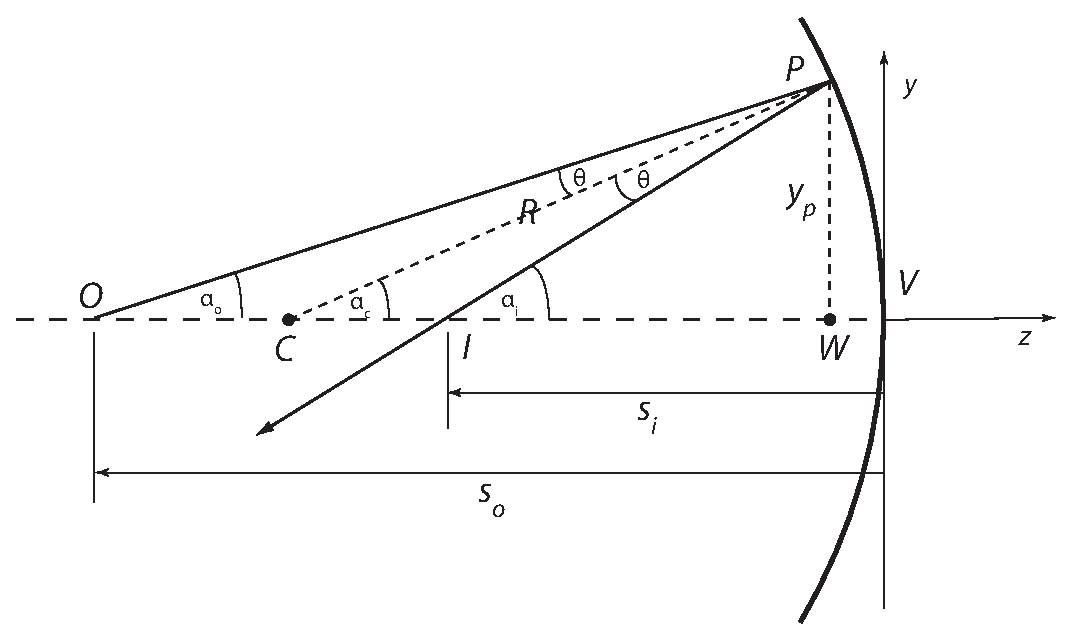
\psfig{file=reflection_spherical.eps,width=0.9\textwidth}\hfil
	\centering
	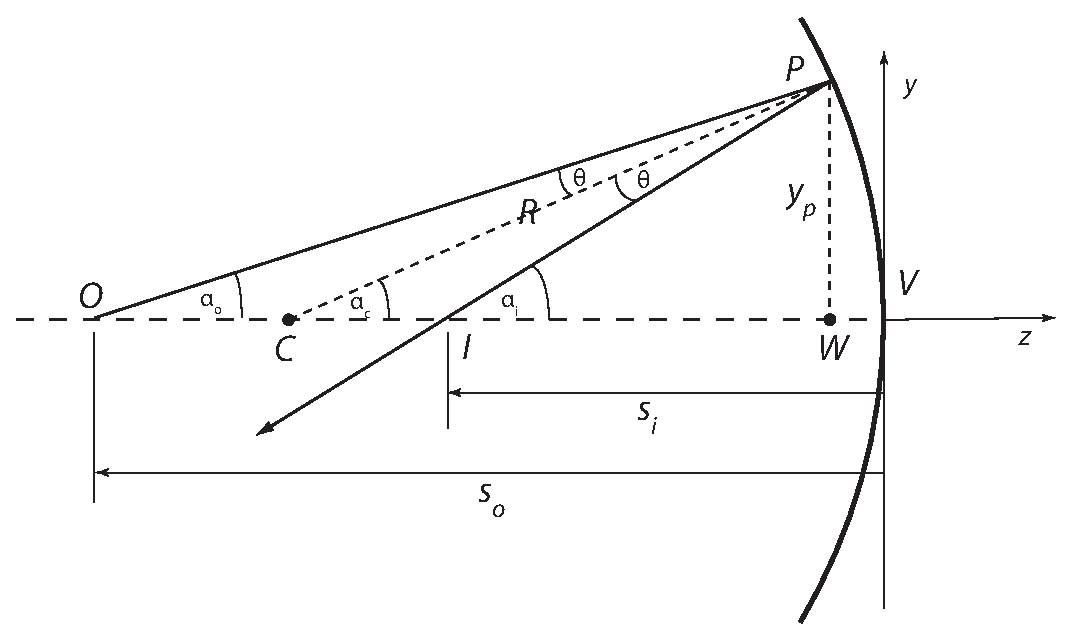
\includegraphics[width=0.9\textwidth]{reflection_spherical.eps}
  \caption{Reflection from a spherical surface. See text for details. }
  \label{fig:reflection_spherical}
\end{figure}

\subsubsection{Reflection from a spherical surface}

Consider a concave spherical surface with radius $R$ and center $C$ as
shown in figure~\ref{fig:reflection_spherical}. The line that is 
coincident with the axis of symmetry (goes through $C$ and the center of the surface)
is called the {\it optical axis}. Set up a Cartesian coordinate system where the $z$-axis
lies on the optical axis and the origin, the {\it vertex} ($V$) is at the point where the surface meets 
the optical axis. Let us describe the situation in the $y-z$ plane. The {\it paraxial approximation}
assumes that all incident rays are nearly parallel to the optical axis, and that all angles
of reflection are small. This latter means that the diameter of the mirror is small compared
to the radius of curvature. 

Consider the ray that originates at the {\it object} at point $O$ on the optical axis and is 
reflected at point $P$ to reach the image at $I$. If the point $P$ is at position $y_p$ then
we can deduce that 
\bua
\alpha_o&\approx&\tan\alpha_o\approx{y_p\over s_o} \\
\alpha_c&\approx&\tan\alpha_c\approx{y_p\over R} \\
\alpha_i&\approx&\tan\alpha_i\approx{y_p\over s_i} 
\eua
given that $s_o$ is the distance between the mirror surface and the object, and $s_i$ is the distance
between the image and the mirror surface (both along the optical axis). The angle $\alpha_c$ is the angle between the line joining the center of the surface $C$ and the point $P$ and the optical
axis.

If $\theta$ is the angle of incidence then we have, considering the triangles $OPC$ and $CPI$ 
that 
\[ 
\theta=\alpha_c-\alpha_o=\alpha_i-\alpha_c
\]
or
\[ 
2\alpha_c=\alpha_o+\alpha_i
\]
Substituting this into the first three approximations for the angles we derive
\[
{2\over R}={1\over s_o}+{1\over s_i}={1\over f}=-P.
\]
The distance $R/2$ is termed the {\it focal length} of the mirror, often written $f$, while
the {\it power} of the surface is written $P$. Note that as the object distance
$s_o$ goes to $\infty$ the image distance $s_i$ goes to $f$.

\subsubsection{Refraction in lenses} % Changed capital letter ``L'' in ``Lenses'' to 'l'.

Snell's law of refraction is also a good starting point for
understanding lenses.
Given that all angles are small, indicies of refraction $n_1,n_2$ and
a radius of curvature $R_{12}$, Snell's law implies that
\[
\frac{n_2}{s_2}-\frac{n_1}{s_1}=\frac{(n_2-n_1)}{R_{12}}.
\]
(note here that $s_1$ is negative).
If we take the focal length $f$ to be the value of $s_2$ when $s_1$
approaches infinity we have
\[
f_2=\frac{n_2R_{12}}{(n_2-n_1)}
\]
Thus, for refraction, the paraxial equation for image and object
distances is
\[
\frac{n_2}{s_2}-\frac{n_1}{s_1}=\frac{n_2}{f_2}=-\frac{n_1}{f_1}=P_{12}
\]
where $P_{12}$ is the {\it power} of the surface. The power, like the
focal length, measures how strongly converging (or diverging for
negative $P$) an interface is. A plane has zero power.

For a lens in air (or vacuum) we can set $n_1=1$ and $n_2=n$ giving the ratio of the speed of light
in vacuum/air to the speed of light in glass, {\it i.e.} $n={c/c_g}$. Snell's 
law implies that a plane wave front in vacuum/air remains plane as light 
enters the glass. A typical value for glass is $1.5$, so the speed of light 
in glass is some $200\,000$~km/s. Since the frequency of light does not change,
this means that the wavelength of light is shorter in glass than in vacuum.

An imaging lens is constructed so that the optical length $w$ in all rays is 
identical even if the geometric distances are different. 

\subsubsection{Imaging properties}

The relation between the distance from a thin lens to an object $s$ and to the 
image of the object $s'$ is related to the focal length $f$ of the lens by the 
thin lens formula
\[
{1\over s}+{1\over s'}={1\over f}
\]

Note that a point infinitely far away is imaged at the focal point of the 
lens, {\it i.e.} that for $s\rightarrow\infty$ then $s'=f$. 

Evaluating an optical design is best done by {\it ray tracing}, {\it
  i.e.} by tracing the path of several rays from an object through all
the optical elements until they form a final image. This is usually
done with a computer program that follows a number of rays, applying
Snell's laws and/or the laws of reflection at every interface ---
usually employing more exact formulations than the paraxial
approximation. However, using the paraxial approximation we can get a
(useful!) rough estimate using only a ruler, paper and a pencil. {\it
  Graphical ray tracing} uses the following specific rules for a thin lens:
\begin{enumerate}
\item Rays incident parallel to the axis emerge through the right
  focal point.
\item Rays incident through the left focal point emerge parallel to the
  axis.
\item Rays through the vertex do not change direction.
\end{enumerate}

{\bf Exercise}

\begin{enumerate}
\setcounter{enumi}{\value{count}}
\item Follow the rules above to make a figure showing the ray tracing
  of  the image of an arrow (lying in the plane of the sky) through a single lens. Indicate the
  positions of the object (the arrow), the focal points, and the image
  of the arrow.
\setcounter{count}{\value{enumi}} 
\end{enumerate}

Likewise, when dealing with a spherical mirror
\begin{enumerate}
\item Incident rays parallel to the optical axis are reflected through
  the focal point, $F$.
\item Incident rays through the focal point are reflected parallel to
  the axis.
\item Incident rays that reach the vertex are reflected back at an
  equal and opposite angle.
\item Incident rays through the center of curvature, $C$, are
  reflected back upon themselves.
\end{enumerate}

{\bf Exercise}

\begin{enumerate}
\setcounter{enumi}{\value{count}}
\item Follow the rules above for a spherical mirror to make a figure showing the ray tracing
  of  the image of an arrow (lying in the plane of the sky). Indicate the
  positions of the object (the arrow), the focal point, and the image
  of the arrow.
\setcounter{count}{\value{enumi}} 
\end{enumerate}

\subsubsection{Simple telescopes}

In its simplest form an astronomical telescope consists of two parts, an 
objective and an eyepiece. The objective images the object one is studying,
and which is ``infinitely'' far away (parallel rays in) on the focal point
or focal plane. This image is real, and can be seen if one places a screen 
in the focal plane. An eyepiece beyond the focal point functions as a 
magnifying glass. These two elements form the basic telescope (see figure~\ref{fig:telescope}).

\begin{figure}[th]
%  \hfil\psfig{file=telescope.eps,width=0.7\textwidth}\hfil
	\centering
	\includegraphics[width=0.7\textwidth]{telescope.eps}
  \caption{Schematic telescope design. Object has angular size $\alpha$ and is focused by 
the primary lens with focal length $F_1$. Image is observed using the eyepiece adjusted so
as to give a virtual image at infinity. The focal length of the eyepiece is $F_0$. }
  \label{fig:telescope}
\end{figure}

The {\it image scale}, $s$, describes the mapping of the sky by any camera. The image scale
is the angular distance on the sky that corresponds to a unit linear distance in the focal 
plane of the camera. Given a focal length $f$, draw paths followed by two rays, one from 
a point ({\it e.g.} a star) on the optical axis, the other from a point separated from the 
first by a small angle $\theta$ on the sky. Rays pass through the vertex without 
deviation, so assuming the paraxial approximation, $\theta\approx\tan\theta$, it is clear that
\[
s={\theta\over y}={1\over f}
\]
where $y$ is the distance the points are separated in the focal plane. Typical focal plane 
detectors are composed of many identical pixels. If the center of each pixel is separated 
from its nearest neighbors by $d$ then the {\it pixel scale} of a telescope is just $s_p=sd$.

{\bf Exercise}

\begin{enumerate}
\setcounter{enumi}{\value{count}}
\item What is the image scale expressed in arcsec per unit lenght?
\setcounter{count}{\value{enumi}} 
\end{enumerate}

The {\it focal ratio} is defined as 
\[
\cl{R}={f\over D}
\]
where $D$ is the diameter of the entrance aperture of the telescope. One can show that the 
brightness (energy per unit area to the focal plane) is proportional to $\cl{R}^2$.

The magnification $M$ of a telescope is given by considering that the image
formed by an object at an angle of $\alpha$ (assumed small) to the optical axis.
The real image is in focus at distance $F_1$, where $F_1$ is the focal length of the
objective lens, since the object is very far away. This image is observed by the eyepiece 
adjusted so as to give a virtual image at infinity, {\it i.e.} the eyepiece should be a distance
$F_0$ away from the image formed by the objective. Considering the geometry of the 
system shown in figure~\ref{fig:telescope} we see that the magnification $M$ must 
be given by $M={\beta/\alpha}$ and that therefore
\[ M={\beta\over\alpha}={\tan({h/F_0})\over\tan({h/F_1})}\approx{{h/F_0}\over{h/F_1}}={F_1\over F_0}.\]
Note that the image is formed upside down.

\subsection{Optical Materials}

An ideal mirror should have a reflectivity of 1.0 for all wavelengths ($\lambda$) of interest. The
substrate should be easy to shape to an accuracy of a fraction of $\lambda$, and once shaped, 
should be mechanically and chemically stable. Low mass is a virtue, as mirrors and lenses should
be as large as possible and must be mobile. Since the temperature can change rapidly high 
thermal conductivity and a low coefficient fo thermal expansion are also essential.

For reflecting telescope's first two centuries, one used {\it speculum metal}, an alloy
primarily of copper and tin. However, it was (is) heavy and only has 45\% reflectivity at best, 
and tarnishes easily. Astronomers therefore switched to silvered glass mirrors once the 
technology became available in the 1880s. Most modern mirrors generally use substrates
made with special glasses ({\it e.g.} Pyrex) or ceramics (Cervit or Zerodur) that have low
coefficients of thermal expansion. A coating of Al is best for the near ultraviolet and optical
since Al is durable and cheap. Ag is poor in the ultraviolet, is superior to Al when 
$\lambda>450$~nm. Au is best in the infrared for $\lambda>650$~nm. Be is toxic, but is the
lowest density workable metal with very good rigidity. 

Short wavelengths, extreme ultraviolet (EUV) and shorter, present
difficulties: First energetic photons tend to be absorbed, scattered,
or transmitted by most materials, and second, curved mirrors in general
need to be shaped with an accuracy of at least $\lambda/4$, which for
a 1~nm X-ray, amounts to one atomic diameter! X-Ray and EUV focusing
telescopes are therefore often designed to operate with grazing
incidence as discussed later.

Transmitting materials form lenses, windows, correctors, prisms, filters, fibres, and more. Of
primary relevance are index of refraction, dispersion, and absorption. The index of refraction for
a number of glasses as a function of wavelength $\lambda$ is shown in table~\ref{tab:glass-refraction}. Generally glasses with a high index of refraction will also have high dispersion and are called ``flints'', while those with smaller index and dispersion are 
called ``crowns''. 

In ultraviolet (150~nm -- 400~nm) ordinary glasses become opaque, fused quartz (SiO$_2$) is
the exception. All other ultraviolet transmitting materials are crystalline, rather than glass, and
are more difficult to shape and more likely to chip and scratch. The most useful is perhaps
calcium fluoride (CaF$_2$), which transmits from 160~nm to 7~$\mu$m. Other fluoride crystals
have similar properties. Fused quartz and fluorides do not transmit well below 180~nm and some
birefringent crystals, such as sapphire (Al$_2$O$_3$) can be used in the very far ultraviolet.
Optics for $\lambda < 150$~nm must be reflecting and for $\lambda < 15$~nm only grazing
incidence reflections are possible.

In the infrared ordinary glasses transmit to about $2.2~\mu$m, and some special glasses to 
$2.7~\mu$m. A large selection of crystalline materials, some identical to those used in the
ultraviolet, transmit to much longer $\lambda$, but most are soft, or fragile, or sensitive to
humidity, so can only be used in protected environments.

% Maybe change table width to fill the textwidth.
\begin{table}
\centering
\begin{tabular}{llllll}
\hline\hline
& & & & & \\
\multicolumn{6}{c}{Refractive index at the specified wavelengths (nm)} \\
Glass type & 361 & 486 & 589 & 656 & 768  \\
\hline
& & & & & \\
Crown & 1.539 & 1.523 & 1.517 & 1.514 & 1.511 \\
High dispersion crown & 1.546 & 1.527 & 1.520 & 1.517 & 1.514 \\
Light flint & 1.614 & 1.585 & 1.575 & 1.571 & 1.567 \\
Dense flint & 1.705 & 1.664 & 1.650 & 1.644 & 1.638 \\
\hline
\end{tabular}
\caption{Index of refraction in various glass types vary as a function
of wavelength and are thus dispersive.}
\label{tab:glass-refraction}
\end{table}

Coating the surface of an optical element with a thin film can exploit
the wave properties of light to increase, or decrease, its
reflectance. A thin film exactly ${1/4}$ wavelength thick applied to a
reflecting substrate will introduce two reflected beams, one from the front film
surface, and the other from film-substrate interface. The second beam
will be emerge one-half wavelength out of phase, and the two beams
will destructively interfere. If the amplitudes are equal, the
interference will be total. An antireflection coating works best at only
one wavelength, but will to some extent also work for a broader band
centered near the design wavelength. A similar technique can enhance
the reflectivity of a surface and multiple layers fo alternating high
and low index materials can improve the reflectivity of a mirror over
a broad range of mirrors. Such {\it multilayer mirrors} are in
frequent use in solar satellites observing the sun at normal incidence
in the EUV as will be discussed later.

\subsection{Chromatic aberration}

Chromatic aberration arises through the change in the refractive index of
glass or other optical material with the wavelength. Typical values for
some optical glasses are shown in table~\ref{tab:glass-refraction}. The 
degree to which the refractive index varies with wavelength is called the 
dispersion, and is measured by the constringence $\nu$
\begin{equation}
\nu={\mu_{589}-1\over\mu_{486}-\mu_{656}}\label{eq:costringence}
\end{equation}
where $\mu_\lambda$ is the refractive index of the wavelength $\lambda$. Note
that the costringence (also called the {\it Abbe number} is roughly inversely 
proportional to the dispersion, {\it i.e} $({dn/d\lambda})$.  The
three wavelengths that are chosen for the definition of $\nu$ are those
of strong Fraunhofer lines: the C-line 486~nm H$\beta$, the D lines 589~nm (Na), 
and the F-line 656~nm H$\alpha$. The glasses listed above have constringence that 
varies from 57 for crown glass to 33 for the dense flint. 

\begin{figure}[th!]
% \hfil\psfig{file=chromatic-aberration.eps,width=0.5\textwidth}\hfil
 \centering
 \includegraphics[width=0.5\textwidth]{chromatic-aberration.eps}
  \caption{Chromatic aberration.}
  \label{fig:chromatic-aberration}
\end{figure}

The effect of dispersion upon an image is to spread it out into a series of
different colored images along the optical axis. Looking at this sequence of
 images with an eyepiece, then at a particular point along the optical axis, the
observed image will consist of a sharp image in the light of one wavelength
surrounded by blurred images of varying sizes in the light of all remaining 
wavelengths. To the eye, the best image occurs when yellow light is focused 
since it is less sensitive to red and blue light.
The spread of colors along the optical axis is called the
{\it longitudinal chromatic aberration}, while that along the image plane
containing the circle of least confusion is called the {\it transverse
chromatic aberration}.

\begin{figure}[th!]
%  \hfil\psfig{file=sst-design.eps,width=0.9\textwidth}\hfil
	\centering
	\includegraphics[width=0.9\textwidth]{sst-design.eps}
  \caption{Schematic drawing of the Swedish 1-meter Solar Telescope tower 
with the turret and vacuum system (center drawing). Details of the box 
holding the field mirror and field lens are shown in A and the Schupmann 
corrector with one lens and one mirror in B. The re-imaging optics, located on
the optical table and consisting of a tip-tilt mirror, an adaptive mirror 
and a re-imaging lens are shown in C.}
  \label{fig:sst-design}
\end{figure}

Delayed by Newton's declaration of impossibility, in the 1760s in France 
and England it was discovered that 
two (or more) lenses can be combined to reduce the effect of chromatic 
aberration. Commonly a biconvex crown glass lens is combined with a 
planoconcave flint glass lens to produce an {\it achromatic doublet}. This can 
reduce the chromatic dispersion by a factor 30. If the radii of the 
curved surfaces are all equal, then the condition for two wavelengths,
$\lambda_1$ and $\lambda_2$, to have coincident images is 
\[
2\Delta\mu_C=\Delta\mu_F
\]
where $\Delta\mu_C$ and $\Delta\mu_F$ are the differences between the 
refractive indices at $\lambda_1$ and $\lambda_2$ for the crown glass and
flint glass respectively. More flexibility in the design can be achieved 
if the two surfaces of the converging lens have differing radii. Then the
condition for achromatism is
\[
{\labs R_1\rabs+\labs R_2\rabs\over\labs R_1\labs}\Delta\mu_C=\Delta\mu_F
\]
where $R_2$ is the radius of the surface of the crown glass that is in 
contact with the flint lens and $R_1$ is the radius of the other surface
of the crown glass lens. Fraunhofer perfected the design and construction
of achromats which led to the possibility of making large refractors, which became 
the telescope design of choice at most observatories after the 1820s.
The era of the refractor came to an end around 1900 when the size of these
reached roughly 1~m, above which size gravity deforms the shape of the lens. It is 
interesting to note that the Swedish 1-meter Solar Telscope with a 1.0~m lens is
one of the worlds largest refractors.

Since photographic film has a different wavelength sensitivity than the
human eye, achromats had to be redesigned when photographic technology 
was adopted by astronomers in the 1880s. 

It is possible to design doublets so that three or more wavelengths are corrected, in this
case the corrective lenses are called {\it apochromats}. Adding more lenses, a properly 
designed {\it triplet}, called a {\it superapochromat} can bring four wavelengths into 
a common focus.

\subsubsection{Schupmann achromat}

Another interesting solution to the problem of achieving an achromatic image
is the combination of a positive lens and a second negative lens in which case
one has an intermediate image and the final image is virtual. This is named
a Schupmann lens. The drawback of the virtual image location can be overcome
with the help of a mirror. The collecting mirror is placed behind the negative
lens, which is used twice and therefore has less power than the negative lens
in the usual setup. There are few refracting telescopes in professional night 
time astronomy, but the Swedish 1-meter Solar Telescope is a refracting 
telescope in which a Schupmann achromat is used.

\subsection{Seidel Aberrations}

\begin{figure}[th!]
%  \psfig{file=aberration_geometry.eps,width=0.95\textwidth}
	\centering
	\includegraphics[width=0.95\textwidth]{aberration_geometry.eps}
  \caption{Geometry used in the Seidel aberration discussion. The left hand
diagram shows rays through the the center of curvature (CFB) and vertex (VV', the chief ray), which
along with the optical axis defines the meridional plane. Point P is outside the plane of the diagram. 
The right hand locates points P, V, and B in the plane of the aperture when looking down the optical axis.}
  \label{fig:aberration-geometry}
\end{figure}

Consider a ``perfect'' telescope, it should transform an incident plane wavefront into
a converging spherical wavefront whose center is the focus predicted by the paraxial 
approximation. For point sources off-axis the perfect telscope should produce spherical
wavefronts converging somewhere on the image plane, also as predicted by the paraxial 
theory. Define the {\it chief ray} as the one passing from the object through the center
of the entrance aperture. The plane containing this ray and the optical axis defines the
{\it meridional} or {\it tangential plane}. The plane perpendicular to this plane is called
the {\it sagittal plane}. If we now analyse the angles of reflection or refraction for a 
curved surface using the approximation 
\[
\sin\theta\approx\theta-{\theta^3\over 3!}
\] 
one obtains {\it third-order aberration theory} which is much more accurate than that
given by paraxial theory where one assumes $\sin\theta=\tan\theta=\theta$. In this 
treatment one can show that the optical path {\it difference} between a test ray and the
chief ray takes the form
\bea{eq:seidel}
\Delta w(\rho,\phi,b)&=&C_1\rho^4+C_2\rho^3b\cos\phi \\
                                &+&C_3\rho^2b^2\cos^2\phi+C_4\rho^2b^2+C_5\rho b^3\cos\phi
\eea
where the $C_i$ values depend on the shapes of the optical surfaces and/or the indices of
refraction. Each of the terms in this equation~\ref{eq:seidel} has a different functional
dependence, so one distinguishes five monochromatic third-order aberrations which are
also known as the {\it Seidel aberrations}. Note that since the range of $\rho$ depends on 
the diameter of the telescope the terms with the highest order of $\rho$ are the most
important.

\subsubsection{Spherical aberration $\propto\rho^4$}

\begin{figure}[th!]
%  \hfil\psfig{file=spherical-aberration.eps,width=0.9\textwidth}\hfil
	\centering
	\includegraphics[width=0.9\textwidth]{spherical-aberration.eps}
  \caption{Spherical aberration.}
  \label{fig:spherical-aberration}
\end{figure}

A common and severe aberration of both lenses and mirrors is {\it spherical 
aberration}: annuli of the lens or mirror that are of different radii have 
different focal lengths. It is possible to minimize but not eliminate spherical
aberration by minimizing the angles of incidence on every surface. Likewise,
any lens with a large enough focal ratio will approach the paraxial case closely enough
that the blur due to spherical aberration can be made smaller than the seeing disk.
Since a large focal ratio also minimizes the chromatic aberration, early refracting telescopes 
(1608 -- 1670) tended to have moderate apertures and large focal lengths, at the cost
of reduced image brightness and unwieldy telescope length.

For mirrors, removing spherical aberration is simple. A paraboloid reflector, 
made by deepening the sphere to a paraboloidal surface, 
will display no on-axis aberrations at all --- rays from infinity parallel to 
the axis will all come to the same focus. Newton constructed the first 
workable reflecting telescope in 1668, and reflecting
telescopes were fashionable from the 1780s (when the Herschels were making great
discoveries with speculum parabaloids) until the superiority of the refractor became
apparent in the 1830s as a result of the discovery that an achromatic doublet can be 
designed to minimize both chromatic aberration and spherical aberration:  
These cannot be
eliminated from a simple lens without using aspheric surfaces, but can be
reduced for a given focal length by adjusting the shape factor $q$
\[
q={R_2+R_1\over R_2-R_1}
\]
where $R_1$ and $R_2$ are the radii of the first and second surfaces 
of the lens respectively. Judicious choice of surface radii in an 
achromatic doublet can lead to some correction of spherical aberration while
still retaining the color correction. 

It is also possible to remove spherical aberration from a {\it spherical} mirror by 
the use of a transparent corrector plate, as we will discuss in connection with
Schmidt and Maksutov telescopes later in this lecture.

%Spherical aberration increases with
%the fourth power of the diameter and inversly proportional to the third 
%power of the focal length.

\subsubsection{Coma $\propto \rho^3b\cos\phi$}

{\it Coma} in an optical system refers to an aberration which results
in off-axis point sources such as stars appearing distorted. Specifically, 
coma is defined as a variation in magnification over the entrance pupil. 
Coma is an inherent property of telescopes using parabolic mirrors, thus
deepening a spherical mirror in order to correct spherical aberration will
introduce coma. It causes the images for objects away from the optical axis
to consist of a series circles that correspond to the various annular 
zones of the lens or mirror and which are progressively shifted away from 
the optical axis. The severity of the coma is proportional to the square of
the aperture and the angular size of the blur is given by
\[ 
L=A{bD^2\over f^3}=A\theta\cl{R}^{-2}
\]
where $A$ is a constant that depends on the shape of the surface.

% Coma is zero in systems that obey Abbe's sine condition
%\[
%{sin\theta\over\sin\phi}={\sin\theta_{\rm p}\over\sin\phi_{\rm
%    p}}\approx{theta_{\rm p}\over\phi_{\rm p}}
%\]
%where the angles are de$\theta$, $\phi$ are the angles relative the optical axis
%of any two rays as they leave the optical system and $\theta_$, $\phi'$ the
%angles of the same rays as they reach the image plane. In other words, 
%the sine of the output angle should be proportional to the sine of the 
%input angle in order to satisfy Abbe's sine condition.

%\begin{figure}[th!]
%  \hfil\psfig{file=abbes-sin.eps,width=0.9\textwidth}\hfil
%  \caption{Angles used in describing Abbe's sine condition.}
%  \label{fig:abbes-sin}
%\end{figure}

Lenses or mirrors in which both spherical aberration and coma are minimized at a single
wavelength are called best form or {\it aplanatic}. No single element aplanatic telescope
is possible, either in a reflector or a refractor. As with spherical aberration, a large
focal ratio will reduce coma, but impose penalties in image brightness and telescope length.
Otherwise, minimizing coma in a refracting system requires a system of lenses, and at least
two mirrors in reflecting telescopes.

\subsubsection{Astigmatism $\propto b^2\rho^2\cos^2\phi$}

\begin{figure}[th!]
%  \hfil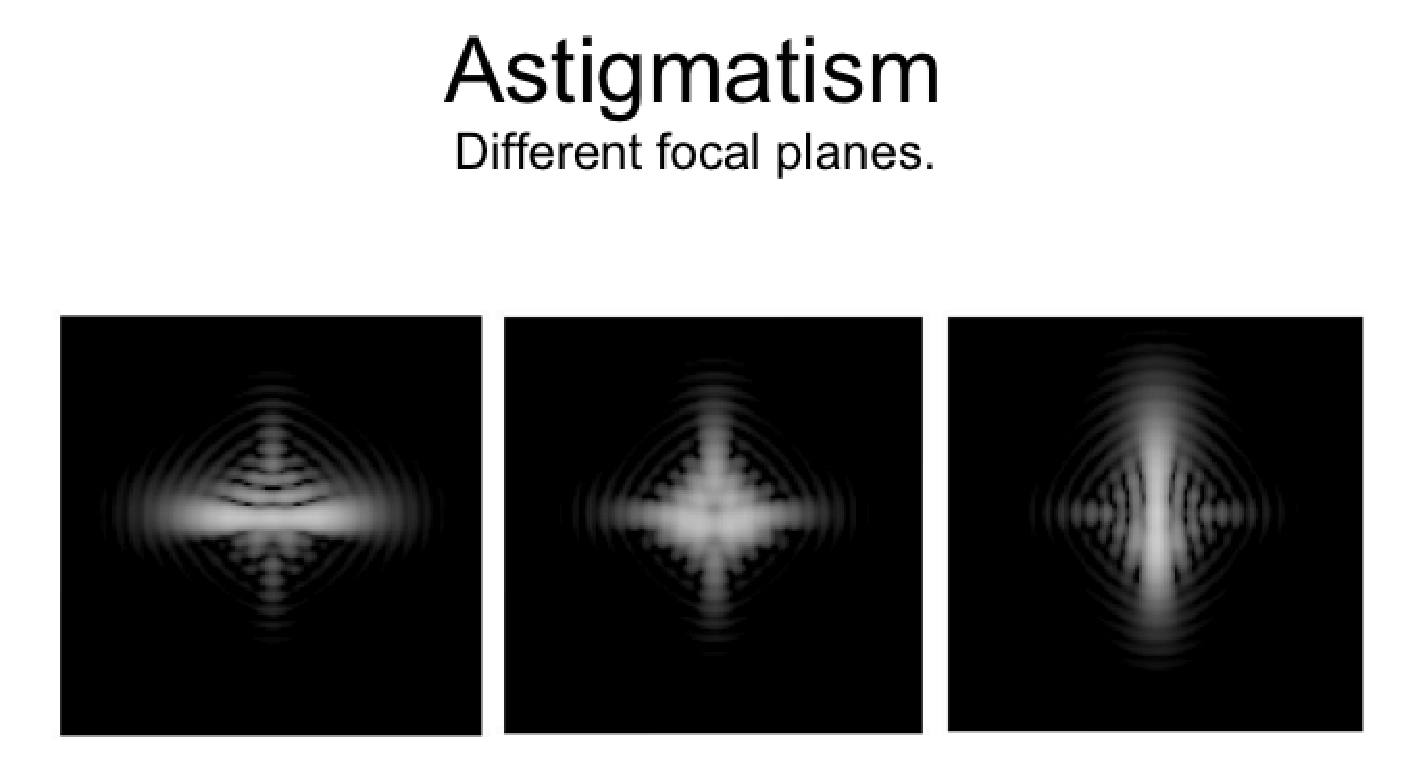
\psfig{file=astigmatism-example.eps,width=0.7\textwidth}\hfil
	\centering
	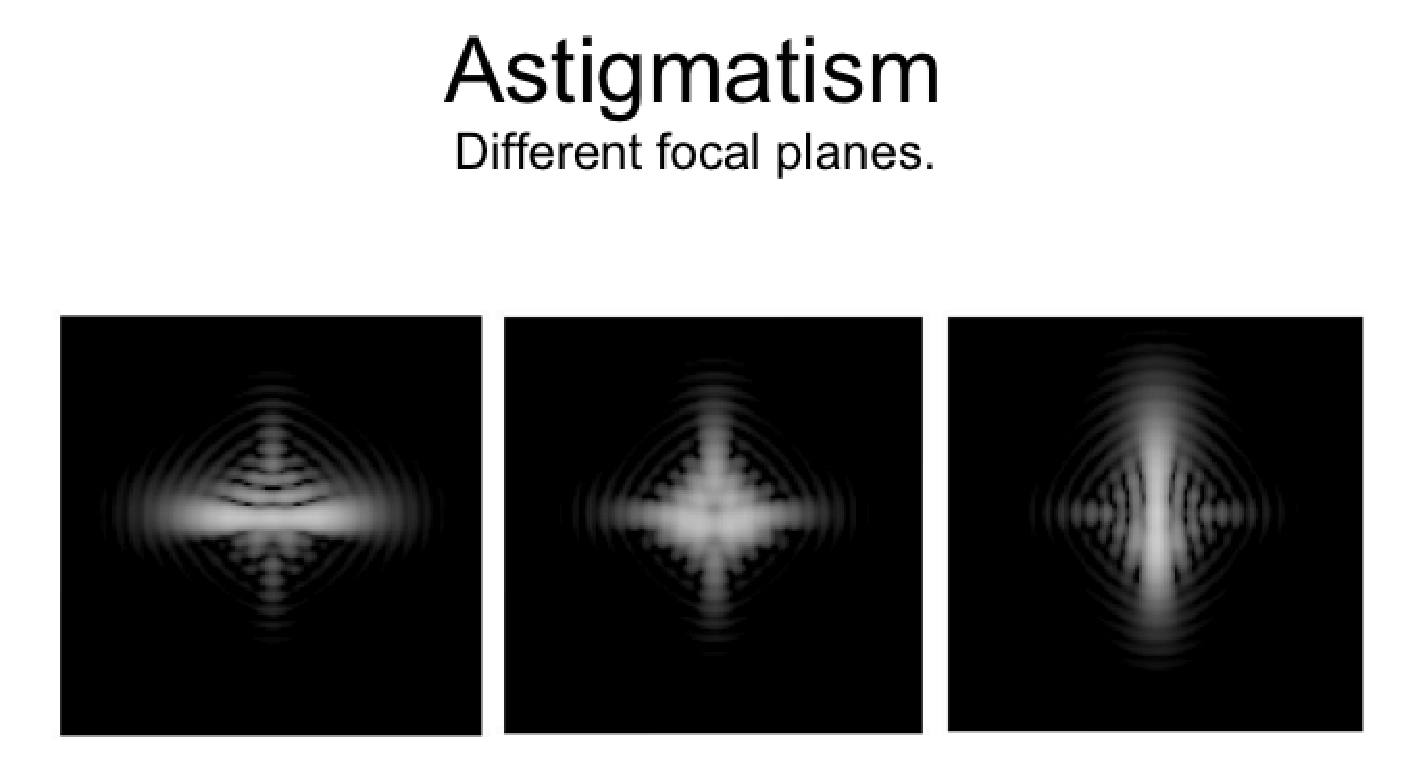
\includegraphics[width=0.7\textwidth]{astigmatism-example.eps}
  \caption{Example of the effect of astigmatism.}
  \label{fig:astigmatism-example}
\end{figure}

{\it Astigmatism} is an effect where the focal length differs for rays in the plane
containing an off-axis object and the optical axis (tangential plane),
in comparison with rays in the plane at right angles to this (sagittal plane).
An example of astigmatism is shown in figure~\ref{fig:astigmatism-example}.
The angular dependence suggests that the wavefront distortion is zero for rays
in the sagittal plane ({\it i.e.} $\phi=90^{\circ}$, $\phi=270^{\circ}$), but an extremum for
rays in the meridional plane.

The blurred image suffering astigmatism has an angular length
\[
L=B\theta^2\cl{R}^{-1}
\]
where $B$ is a constant that depends on the shape of the reflecting or refracting surface.

It is possible to correct astigmatism, but at the expense of introducing
an aberration called field curvature, {\it i.e.} that the surfaced containing
the sharply focused image is not flat but curved. A system where a flat 
image plane is combined with corrected astigmatism is termed {\it anastigmatic}
and a telescope that corrects for astigmatism, coma, and spherical aberration a
anastigmatic aplanat. 

\subsubsection{Field curvature $\propto\rho^2 b^2$}

This aberration results from off-axis images falling on a spherical surface called the
{\it Petzval surface}. Detectors are generally flat, so much of an image formed on a 
detector will be out of focus. For a small detector, this defocus will not exceed the 
seeing disk or diffraction limit and therefore not be a problem. For larger detectors
is to bend the detector to fit the Petzvel surface, as was done with photographic plates
using a mechanical plate holder. Large solid-state detectors like CCDs are mechanically 
quite fragile, so bending is not an option. In which case a corrector plate or lens is
used to flatten the field.

\subsubsection{Distortion $\propto \rho b^3\cos\phi$}

\begin{figure}[th!]
%  \hfil\psfig{file=aberration-distort.eps,width=0.9\textwidth}\hfil
	\centering
	\includegraphics[width=0.9\textwidth]{aberration-distort.eps}
  \caption{Distortion}
  \label{fig:aberration-distortion}
\end{figure}

The final aberration is {\it distortion}, which is a variation in the 
magnification over the image plane. A distorted system will deliver images
that suffer {\it pincushion} or {\it barrel} distortion according to 
whether the magnification increases or decreases with distance from the 
optical axis.

Since distortion does not change the image quality, it can be removed from 
digital in a post processing phase.

Another fault of optical systems is called {\it vignetting}. It arises as a result
of uneven illumination of the image plane, usually due to the obstruction of 
the light path by parts of the instrument.

\subsubsection{Zernike polynomials}

\begin{figure}[th!]
%  \hfil\psfig{file=zernike_polynomials.eps,width=0.4\textwidth}\hfil
	\centering
	\includegraphics[width=0.4\textwidth]{zernike_polynomials.eps}
  \caption{The first few Zernike polynomials, see table~\ref{tab:zernike-polynomials} 
}
 \label{fig:zernike-polynomials}
\end{figure}

% Do something about the table. Too wide for the paragraph. Might change if book is used.
\begin{table}
\begin{tabular}{ll}
\hline\hline
&  \\
\multicolumn{2}{c}{Roles of the Zernike polynomials} \\
&  \\
$a_0$ & ``Piston'', equal to the mean value of the wavefront \\
$a_1\times\rho\cos(\varphi)$ & ``X-tilt'', the deviation of the overall beam in the sagittal direction \\
$a_2\times\rho\sin(\varphi)$ & ``Y-tilt'', the deviation of the overall beam in the tangential direction \\
$a_3\times(2\rho^2-1)$ & ``Defocus'', a parabolic wavefront resulting from being out of focus \\
$a_4\times\rho^2\cos(2\varphi)$ & ``X-astigmatism'', horizontally oriented cylindrical shape \\
$a_5\times\rho^2\sin(2\varphi)$ & ``Y-astigmatism'', vertically oriented cylindrical shape \\
$a_6\times(3\rho^2-2)\rho\cos(\varphi)$ & ``X-coma'', comatic image flaring in the horizontal direction \\
$a_7\times(3\rho^2-2)\rho\sin(\varphi)$ & ``Y-coma'', comatic image flaring in the vertical direction \\
$a_8\times(6\rho^4-6\rho^2+1)$ & ``Third order spherical aberration'' \\
\hline
\end{tabular}
\caption
{$\rho$ is the normalized pupil radius, $\varphi$ is the azimuthal angle around the pupil,
the coefficient $a_0,\ldots,a_8$ are the wavefront errors in wavelengths.}
\label{tab:zernike-polynomials}
\end{table}

In an optical system the location of the diffraction focus will depend
on the type and magnitude of aberration present. Because of this
dependence, it is appropriate to restructure the classical aberration
terms and include explicitly the required image shift to place the
diffraction focus at the origin. These modified terms are called the
orthogonal aberrations, with polynomials in $\rho$ and $\varphi$ ({\it
  i.e.} using a circular co-ordinate system) called
{\it Zernike polynomials}. Developed by Frits Zernike in the 1930s,
 Zernike's polynomials are orthogonal over a circle of unit radius. A complex, 
aberrated wavefront profile may be curve-fitted with Zernike polynomials to 
yield a set of fitting coefficients that individually represent different 
types of aberrations. Their advantage are the simple analytical
properties which leads to closed form expressions of the
two-dimensional Fourier transform in terms of Bessel functions. 
Their disadvantage, in particular for high $n$ is the unequal
distribution of nodal lines over the unit disk, which introduces
ringing effects near the perimeter $\rho\approx 1$, which leads
attempts to define other orthogonal functions over the circular 
disk\footnote{For atmospheric turbulence
  Zernike polynomials are not the optimal set of basis functions
  because the Zernike coefficients are statistically dependent. Basis
  functions that do not have this property can be constructed and are
  called the {\it Karhunen--Lo{\'e}ve functions} which represent
stochastic processes as an infinite linear combination of orthogonal
functions analogous to a Fourier series representation of a function
on a bounded interval. The coefficients in the Karhunen--Lo{\'e}ve
theorem are random variables and the expansion basis depends on the
process. The Karhunen--Lo{\'e}ve transform adapts to the process in 
order to produce the best possible basis for its expansion. (Source: 
Wikipedia and Gua-ming Dai {\it Modal compensation of atmospheric
  turbulence with the use of Zernike polynomials and
  Karhunen-Lo{\'e}ve functions} J.Opt.Soc.Am. 12, October 1995.)}.

There are even and odd Zernike polynomials. The even ones are defined as
\[
Z_n^m(\rho,\varphi)=R_n^m(\rho)\cos(m\varphi)
\]
and the odd ones
\[
Z_n^{-m}(\rho,\varphi)=R_n^m(\rho)\sin(m\varphi)
\]
where $m$ and $n$ are non-negative integers with $n\ge m$, $\varphi$ is the
azimuthal angle and $\rho$ is the normalized radial distance. The radial 
polynomials $R_n^m$ are defined as
\[
R_n^m(\rho)=\sum_{k=0}^{(n-m)/2}{(-1)^k(n-k)!\over 
   k![{(n+m)/2}-k]![{(n-m)/2}-k]!}\rho^{n-2k}\qquad{\rm if}~n-m~{\rm even}
\]
\[
R_n^m(\rho)=0\qquad{\rm if}~n-m~{\rm odd}
\]

The first few few Zernike polynomials are described in table~\ref{tab:zernike-polynomials}.

\subsection{Practical telescopes}

Even after a telescope design has been perfected; in which one attempts to 
remove as many of the aberrations as possible from the list above, there 
remains the task of physically producing the instrument specified. This must
be done taking into consideration what one actually needs to observe in 
order to meet a certain scientific goals. 

Manufacturing of lenses and mirrors is broadly similar: the surface is roughly
shaped by moulding or diamond milling. It is then matched to another surface
formed in the same material whose shape is inverse, called the {\it tool}. 
The two surfaces are ground together with coarse carborundum or other grinding
powder between them until the required surface begins to approach 
its specifications. The pits left behind are removed by a second grinding stage
in which finer powder is used. A third stage follows, and so on. As many as
eight or ten such stages may be necessary. When grinding pits are reduced to
a micron or so in size, the surface may be polished. Once the surface has been
polished it can be tested for accuracy of fit. A third stage termed {\it 
figuring} is often necessary when the surface is not within specification. 

There are a number of tests that can determine the shape of a mirror's surface
to within $\pm 50$~nm or better, such as Foucault, Ronchi, Hartmann and Null
tests. 

\noindent
{\it Epicyclic grinding.} Larger mirrors are ground by using large machines that 
move the tool in an epicyclic fashion. The motion of the tool is similar to that of 
the planets under the Ptolemaic model of the solar system. The epicyclic motion 
can be produced by a mechanical arrangement, but commercial production of 
large mirrors is now largely done by computer controlled planetary polishers. 

\noindent
{\it Stressed polishing.} The mirror segments for large instruments such as the 10~m
Keck or Gran Tecan telescopes are small, off-axis parts of the total hyperbolic shape. 
These are produced by so-called stressed polishing where the blank is is deformed 
by carefully designed forces from a warping harness, and then polished to a spherical
shape. When the the deforming forces are released the blank springs into the required 
shape.

\noindent
{\it Numerically controlled diamond milling.} The requirements for for non-axisymmetric
mirrors for segmented mirror telescopes and and for glancing incidence x-ray telescopes
have led to the development of numerically controlled diamond milling machines which 
can produce the required shaped and polished surface directly to an accuracy of 10~nm or
better.

The defects in an image that are due to surface imperfections on a mirror will
not exceed the Rayleigh limit if those imperfections are less than 
one eighth of the wavelength of the radiation for which the mirror is intended.
The restriction on lenses is about twice as large as those of a mirror
since the ray deflection is distributed over two faces. 

The surface must normally receive its reflecting coating after production. The
vast majority of astronomical mirror surfaces have a thin layer of aluminium
evaporated on to them by heating aluminium wires suspended over the mirror 
inside a vacuum chamber. Other materials such a silicon carbide are sometimes
used, especially for UV since the reflectivity of aluminium falls for 
$<300$~nm. Aluminium initially has a reflectivity of 90~\%, but this will
fall to 75~\% in the matter of months, hence realuminaization is need 
regularly. Mirrors coated with suitably protected silver can achieve 99.9~\%
reflectivity in the visible, and this may be required as the total number of
reflections becomes large.

\noindent
{\it Coefficient of thermal expansion.} To avoid deformations of its shape It is essential
that the coefficient of thermal expansion for a mirror is low. For glass it is of order
$9\times 10^{-6}$~K${-1}$, for pyrex $3\times 10^{-6}$~K${-1}$, and for fused quartz
$4\times 10^{-7}$~K${-1}$. Pyrex has been the favorite material up until the last 30 years
when quartz or artificial materials such as `CerVit' or `Zerodur'. Another possibility is to 
use materials with a very high thermal conductivity, such as silicon carbide, graphite epoxy,
steel beryllium, or aluminium. However, it can be very difficult to polish these materials as
they have a relatively coarse crystalline surface.

\noindent
{\it Rigidity of mirrors, thin mirrors and honeycomb mirrors.} Small solid mirrors can maintain
their shape simply by mechanical rigidity. However, the thickness required for such rigidity
scales as the cube of the size, so the weight of a solid mirror scales as $D^5$ --- this quickly 
becomes to expensive to build. There are various ways to reduce the weight of mirrors, these
fall into two major classes: thin mirrors and honeycomb mirrors. Thin mirrors are also subdivided
into monolithic and segmented mirrors. In both cases active support is needed in order to 
maintain the correct shape. Honeycomb mirrors are thick sold blanks that have had a lot of
the material behind the reflecting surface removed, leaving only thin struts to support that surface. 

\noindent
{\it Rotating mirrors, bath of mercury.} Isaac Newton realized that the surface of a steadily rotating liquid would take up a paraboloidal shape under the combined forces of gravity and
centrifugal acceleration. If the liquid reflects light, like mercury, gallium, gallium-indium alloy, or an oil suffused with reflecting particles, one can then use it as the primary mirror of a telescope. 

\subsubsection{Designs}

The most common format for large telescopes is the Cassegrain system, although
most large telescopes can be usually be used in several alternative 
different modes by interchanging the secondary mirrors. The Cassegrain is
based on a paraboloidal primary and a convex hyperboloidal secondary. The 
major advantage of the Cassegrain lies in its telephoto characteristic, 
the secondary mirror serves to expand the beam from the primary mirror so 
that the effective focal length of the whole system is several times the
that of the primary. A compact (thus cheap) mounting can thus be used to 
hold the optical elements while retaining the advantages of long focal length
and large image scale. The Cassegrain is affiliated with coma and spherical
aberration to about the same degree as an equivalent Newtonian.

\begin{figure}[th!]
%\hfil{
%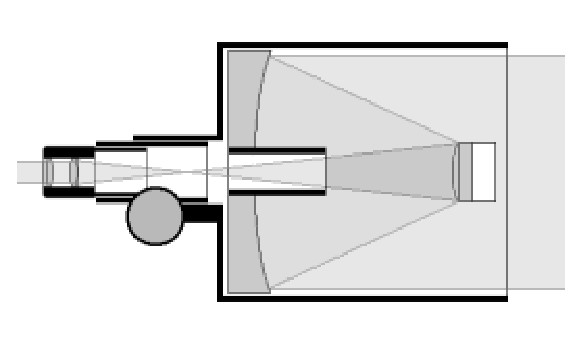
\psfig{file=cassegraindetailed.eps,width=0.45\textwidth}\hfil
%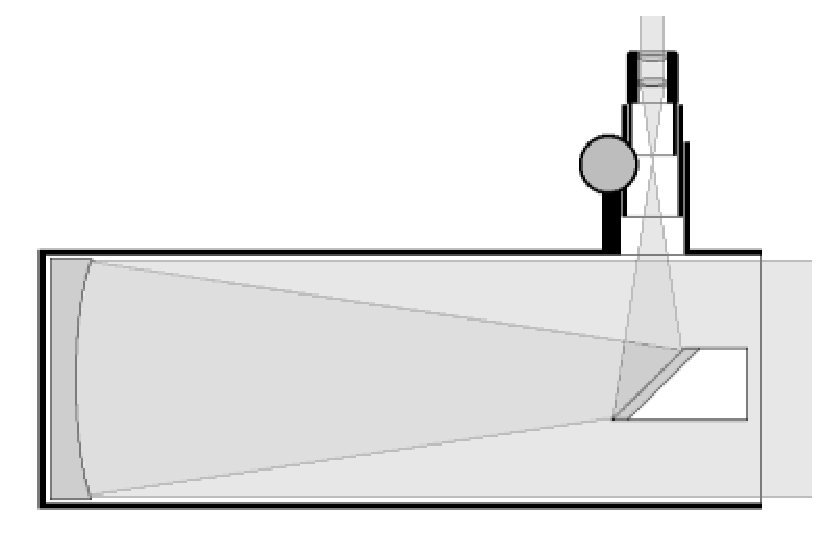
\psfig{file=newtoniandetailed.eps,width=0.45\textwidth}
%}\hfil
	\centering
	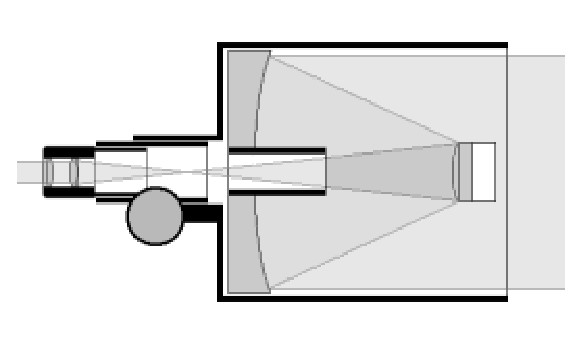
\includegraphics[width=0.45\textwidth]{cassegraindetailed.eps}
	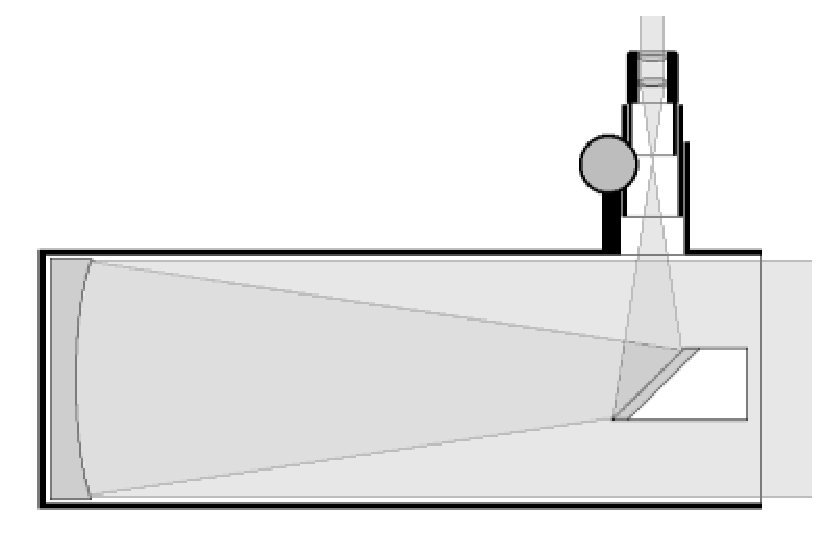
\includegraphics[width=0.45\textwidth]{newtoniandetailed.eps}
  \caption{Cassegrain and Newtonian Designs}
  \label{fig:catatropic}
\end{figure}

A great improvement of the Cassegrain can be achieved by a slight alteration
to a Ritchey-Chr{\'e}tien system. The optical arrangement is identical but for
that the primary mirror is deepened to a hyperboloid and a stronger 
hyperboloid is used for the secondary. With this system both coma and 
spherical aberration can be corrected and one achieves a aplanatic system. 

\noindent
{\it Corrector lenses just before the focus.} One can also improve Cassegrain
or Ritchey-Chr\'etien systems by adding correctors just before the focus. 
The correctors are low power lenses whose aberrations oppose those of the main
system. The corrective optics may be combined with a focal reducer to enable 
the increased field of view to by covered by the detector array. A focal reducer
is a positive lens, usually a apochromatic triplet, placed just before the focal 
point of the telescope that decreases the effective focal length and so gives 
a smaller image scale.

{\it Coud\'e focus.} Another related telescope design is the Coud{\'e} system, which in effect
is a very long focal length Cassegrain or Ritchey-Chr{\'e}tien whose light 
beam is folded and guided by additional flat mirrors to give a focus whose
position is fixed irrespective of the telescope position. One way is to insert a 
diagonal mirror after the secondary, light is reflected down the declination, and 
then down the polar axis by a second diagonal mirror. LIght then always emerges
from the end of the polar axis, whatever part of the sky the telescope is inspecting.

\noindent
{\it Nasmyth focus/system.} With alt-ax mountings the light beam can be directed
along the altitude axis to one of the two Nasmyth foci on the side of the mounting.
These foci still rotate as the telescope changes azimuth, but this is still easier than 
changing the altitude and altitude of a conventional Cassegrain focus. Both of the
fixed focus systems, Coud\'e and Nasmyth, are very advantageous when large equipment
such as high dispersion spectrographs, are to be used. Disadvantages are that the
field of view rotates as the telescope tracks an object across the sky, and is very 
small due to the large effective focal ratios that are required to bring the focus 
through the axes, and finally the additional reflections cause the loss of light.

The simplest of all designs is a mirror used at its prime focus. That is, 
the primary mirror is used directly to produce the images and the detector
is placed at the top end of the telescope. The image quality of at the prime
focus is usually poor even a few tens of arcsec away from the optical axis
because the primary mirrors focal ratio may be as short as f3 or less in
order to reduce the instrument length. A system that is almost identical
to the use of a telescope at prime focus is the Newtonian. A secondary 
flat secondary mirror is used just before the prime focus. This reflects the
light beam to the side of the telescope from where access to it is relatively
simple. There is little advantage to this design over use of the prime focus
for large telescopes. The images in a Newtonian system and at prime focus 
are very similar and are of poor quality away from the optical axis.

A Gregorian is similar to the Cassegrain except that the secondary is a
concave ellipsoid and is placed after the prime focus. Since the primary 
mirror creates an actual image before the secondary mirror, the design
allows for a field stop to be placed at this location, so that the light from outside
the field of view does not reach the secondary mirror. This is a major advantage
to solar telescopes, where a field stop can reduce the amount of heat reaching secondary
mirror and subsequent components. Hinode/SOT (Solar Optical Telscope) is an 
example of a Gregorian.

{\it Refractors (and the Swedish 1-meter Solar Telescope).}

\begin{figure}[th!]
%\hfil{
%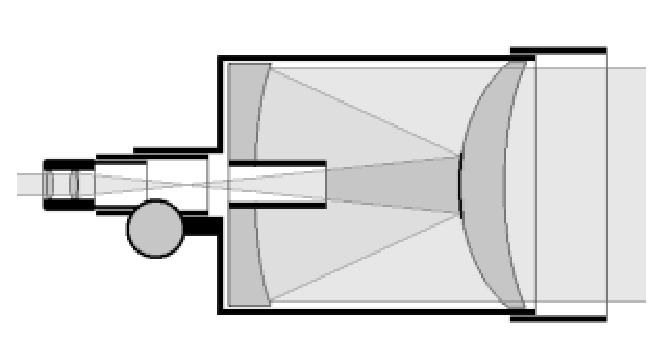
\psfig{file=maksutovcassegraindetailed.eps,width=0.45\textwidth}
%\hfil
%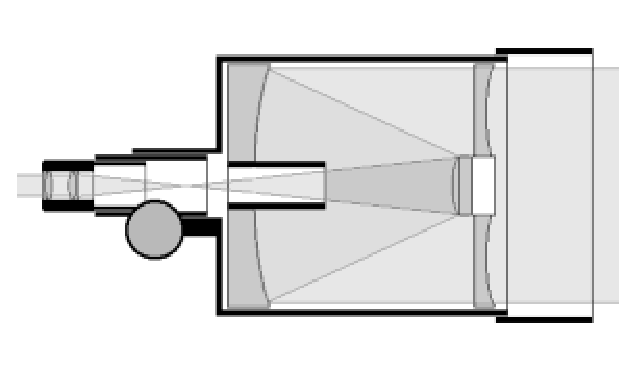
\psfig{file=schmidtcassegraindetailed.eps,width=0.45\textwidth}
%}\hfil
	\centering
	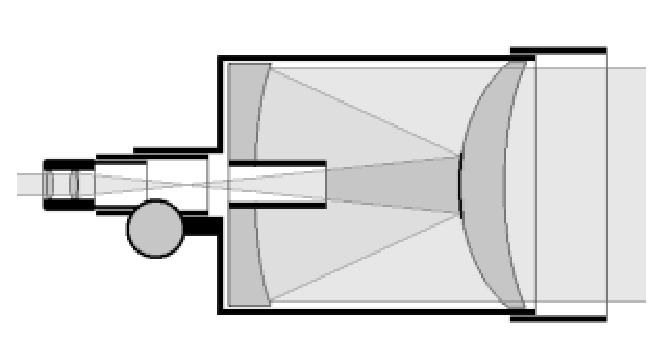
\includegraphics[width=0.45\textwidth]{maksutovcassegraindetailed.eps}
	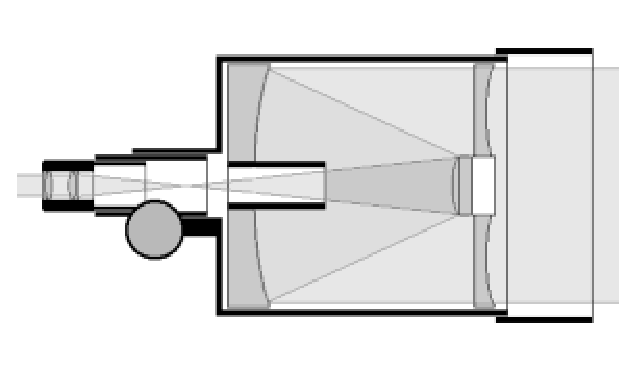
\includegraphics[width=0.45\textwidth]{schmidtcassegraindetailed.eps}
  \caption{Maksutov and Schmidt-Cassegrain Designs}
  \label{fig:catadiotropic}
\end{figure}

The catadioptric (from catoptric, {\it ie} reflecting, and dioptric, {\it ie} 
refracting) group of which the Schmidt camera is best known. A catadioptric 
system uses both lenses and mirrors in its primary light gathering section.
Very high degrees of corrections of the aberrations can be achieved because
of the wide range of variable parameters that become available. Diffraction
limited performance over fields of view of several degrees is possible with
focal ratios as fast as $f1.5$ or $f2$. The Schmidt
camera cannot be used visually since its focus is inaccessible. One of the best
modifications of this is the Maksutov. A similar system is the 
Schmidt-Cassegrain telescope. 

\subsubsection{Mountings}

The functions of a telescope mounting are to hold the optical components 
in their correct mutual alignment, and to direct the optical axis towards the
object to be observed. One can consider the functions of the mounting under 
three separate aspects: supporting the optical components, preserving their 
correct spatial relationship, and acquiring and holding the object of interest 
in the field of view.

\noindent
{\it Equatorial mounting.} This is a two axis mounting, with one axis, the polar axis,
aligned parallel with the Earth's rotational axis, and the other, the declination axis,
perpendicular to the polar axis. Only a single constant velocity motor is required 
to rotate the mounting around the polar axis in order to track an object.

\noindent
{\it Alt-az mounting.} This mounting has motions in altitude and azimuth. Structurally 
it is much simpler and much more compact than the equatorial system. Its drawbacks are 
that the field of view
rotates telescope motion, and that it needs driving continuously in both axes and with 
variable speeds in order to track an object. 

\noindent
{\it Fixed position telescopes.} Some telescopes do not track: {\it e.g.} transit telescopes
point only along the meridian. Other telescopes do not vary their pointing at all and
the tracking function is realized by moving the detector in the image plane while the 
massive telescope remains stationary.

\noindent
{\it Coelostat and heliostat.} A coelostat is comprised of two flat mirrors that are driven 
so that a beam of light from any part of the sky is routed into a fixed direction. They are
particularly used in conjunction with solar telescopes whose extremely long focal lengths
make them impossible to move. One mirror of the coelostat is mounted on a polar axis and
driven at half the sidereal rate. The second mirror is mounted and driven to reflect the light
into the fixed telescope.

\noindent
{\it Mountings in space.} Telescopes in space must also mount and track but since the 
effects of gravity are much less some aspects of these tasks is easier. In general two methods
are used to stabilize the orientation of a telescope in space: small rockets and spinning 
reaction wheels. A space telescope often has more stringent pointing requirements than
a telescope on the ground, and a guide star is often used to achieve this precision. To point
on a given target requires continuous telescope movement because of the aberration of 
starlight induced by the telescopes orbital velocity and because of torques induced by 
atmospheric drag and thermal effects. 

\subsubsection{Telescopes in space}

In connection with a RAND project in 1946, Lyman Spitzer was asked to consider the advantages
of putting an astronomical telescope in space. This work came to full fruition in 1990 
when the Hubble Space Telescope (HST) was launched. The HST has an aperture of 2.4~m and
has generated unprecedented results, revolutionizing astronomy. Its replacement is meant to
be the 6.5~m James Webb Space Telescope (JWST) built by NASA and ESA in collaboration and to
be placed at the Sun-Earth L$_2$ Lagrange point in 2017 (or so).

The absence of an atmosphere and hence wavefront distortions means that a space telescope 
should have diffraction limited resolution. {\it I.e.} that the ``diameter'' of a star will
be of order the Airy disk
\[
\theta={2.44\lambda\over D}
\]
where $\lambda$ is the wavelength observed and $D$ the diameter of the telscope. Since there
are no other distortions, the precision and alignment of optical surfaces becomes especially 
critical in space, where seeing will not mask any errors.

Note that the Earth's atmosphere is itself a source of background light, so from space the
background is lower than on the ground. On the ground there are several sources: {\it 
airglow} (atomic and molecular line emission from the upper atmosphere), scattered sunlight,
starlight and moonlight, and scattered artificial light. In the infrared, the atmosphere and
telescopes both glow like blackbodies and dominate the background. From space the main
contributor in the visible and in the near infra-red (NIR) comes from sunlight scattered from 
interplanetary dust (visible in dark sites on the ground as {\it zodiacal light}.) In the 
V band, the darkest background for the HST (near the ecliptic poles) is about 
23.3~magnitudes/arcsec$^2$, while at the darkest ground based site it is of order 
22.0~magnitudes/arcsec$^2$. In the thermal infrared the sky from space can be much darker than 
on the ground because it is possible to keep the telescope quite cold in space.

The atmospheric absorbes light at certain wavelengths, at these wavelengths it is only possible
to observe from space. This is especially true for gamma-ray, x-ray, and UV astronomy, but also
at other wavelengths: the atmosphere is a dynamic system and weather happens! Astronomers
are often happy to achieve 1\% accuracy on the ground, from space photometry precise to
one part in $10^5$ is possible.

A space telescope in an orbit far enough away from the Earth (and the Moon) also has access 
to the entire sky all the time, half the sky is not blocked by the Earth at any given time, 
nor is a space telescope hindered by the day-night cycle or by moonlight.

A telescope on the ground experiences changing gravitational stresses as in points in different
directions, and will respond by changing shape. Stresses induced by wind and temperature changes
generate similar problems. Most of the expense of a large modern telescope is not in the optics, 
but in the systems needed to move and shelter the optics, while maintaining figure and alignment.

However, the total optical/infrared aperture on the ground exceeds that in space by a factor of
at least 200, and that factor is likely to increase in the near future. The disadvantages of
space astronomy are led by its enormous cost. Typically the two 8~m Gemini telescopes had a 
construction budget of 100~MUSD, the 2.4~m HST cost 2000~MUSD to construct and launch.

\subsubsection{Observatory engineering}

\begin{enumerate}
\item The location of an observatory is vital to its success. Seeing is substantially better
at high altitude on isolated islands like Mauna Kea and La Palma and the various sites in 
northern Chile. 
\item Lightweight mirrors in a compact structure are cost effective. Modern primary mirrors
have fast focal ratios: f/1.75 for Keck, f/3.3 for Hale, which means shorter telescope length 
and a smaller building. The same is true for altazimuth mounts compared to equatorial mounts.
\item Active optics can improve image quality.
\item Local climate control can improve natural seeing. Structures that permit substantial
airflow with {\it e.g.} fans, louvres, retractable panels, while still protecting from 
wind buffeting can improve seeing appreciably.
\item Novel focal arrangements can reduce costs of specialized telescopes. Keck and VLT can 
combine beams from several telescopes at a common focus ({\it i.e} interferometry).
\item Adaptive optics can eliminate some of the effects of atmospheric seeing.
\end{enumerate}

\subsubsection{Future telescopes}

If adaptive optics can produce a large diffraction limited FOV, then current mirror and
mounting technology can allow telescopes of up to 100~m diameters. At present (2010)
there are three serious multinational projects to build single aperture telescopes larger 
than the currently operational 8 -- 11~m instruments. All three projects expect to see 
first light around 2018; and include the European Extremely Large Telescope 
({\tt www.eso.org/sci/facilities/eelt}) with a 
primary of $D=42$~m built up of 1000 1.4~m segments, the Giant Magellan Telescope
({\tt www.gmto.org})
$D=24.5$~m of 7 8.4~m segments, and the Thirty Meter Telescope 
({\tt www.tmt.org})
$D=30$~m consisting of 492 1.4~m segments. Each of these telescopes has a cost of
some $10^9$ US dollars.

%\end{document}
